\label{organ}
%insert organization, schedule and cost estimates here

\subsection{Organization}

Construction and operation of the DUNE-PT is an integrated effort within the experimental program of the DUNE collaboration.  
The DUNE Collaboration management team includes the collaboration Co-Spokespersons, Andre Rubbia (ETH Zurich) and Mark Thomson 
(Cambridge University); the Technical Coordinator, Eric James (Fermilab); and the Resource Coordinator, Chang Kee Jung (Stony 
Brook University).  This team is responsible for coordinating the international effort required to design, construct, install, 
commission, and operate the detectors needed to achieve the scientific objectives of the DUNE Collaboration.  

The DUNE-PT is an integral part of this effort.  This detector will be built from full-scale components and designed to replicate 
the configuration of the first 10~kt detector module to be installed at the Sanford Underground Research Facility (SURF) in 
South Dakota during the early 2020s.  Successful construction and operation of the DUNE-PT will validate the design of this much 
larger detector, and the accomplishment of these tasks is among the highest priorities for the DUNE Collaboration over the 
timescale of the next few years.  Additionally, the subsequent collection and analysis of test beam data from the DUNE-PT will 
provide vital calibration data necessary to achieve its scientific goals.

In addition to taking responsibility for the construction and operation of the DUNE-PT, the DUNE collaboration strongly endorses 
the already approved dual-phase liquid argon detector development program at CERN (WA105 experiment), recognizing the potential 
advantages of this detector technology, which may ultimately be chosen for one or more of the three additional 10~kt detector 
modules to be installed at SURF.     

The organization of the DUNE collaboration is shown in Fig.~\ref{fig:DuneOrg}.  
%
\begin{figure}[htb]
  \centering
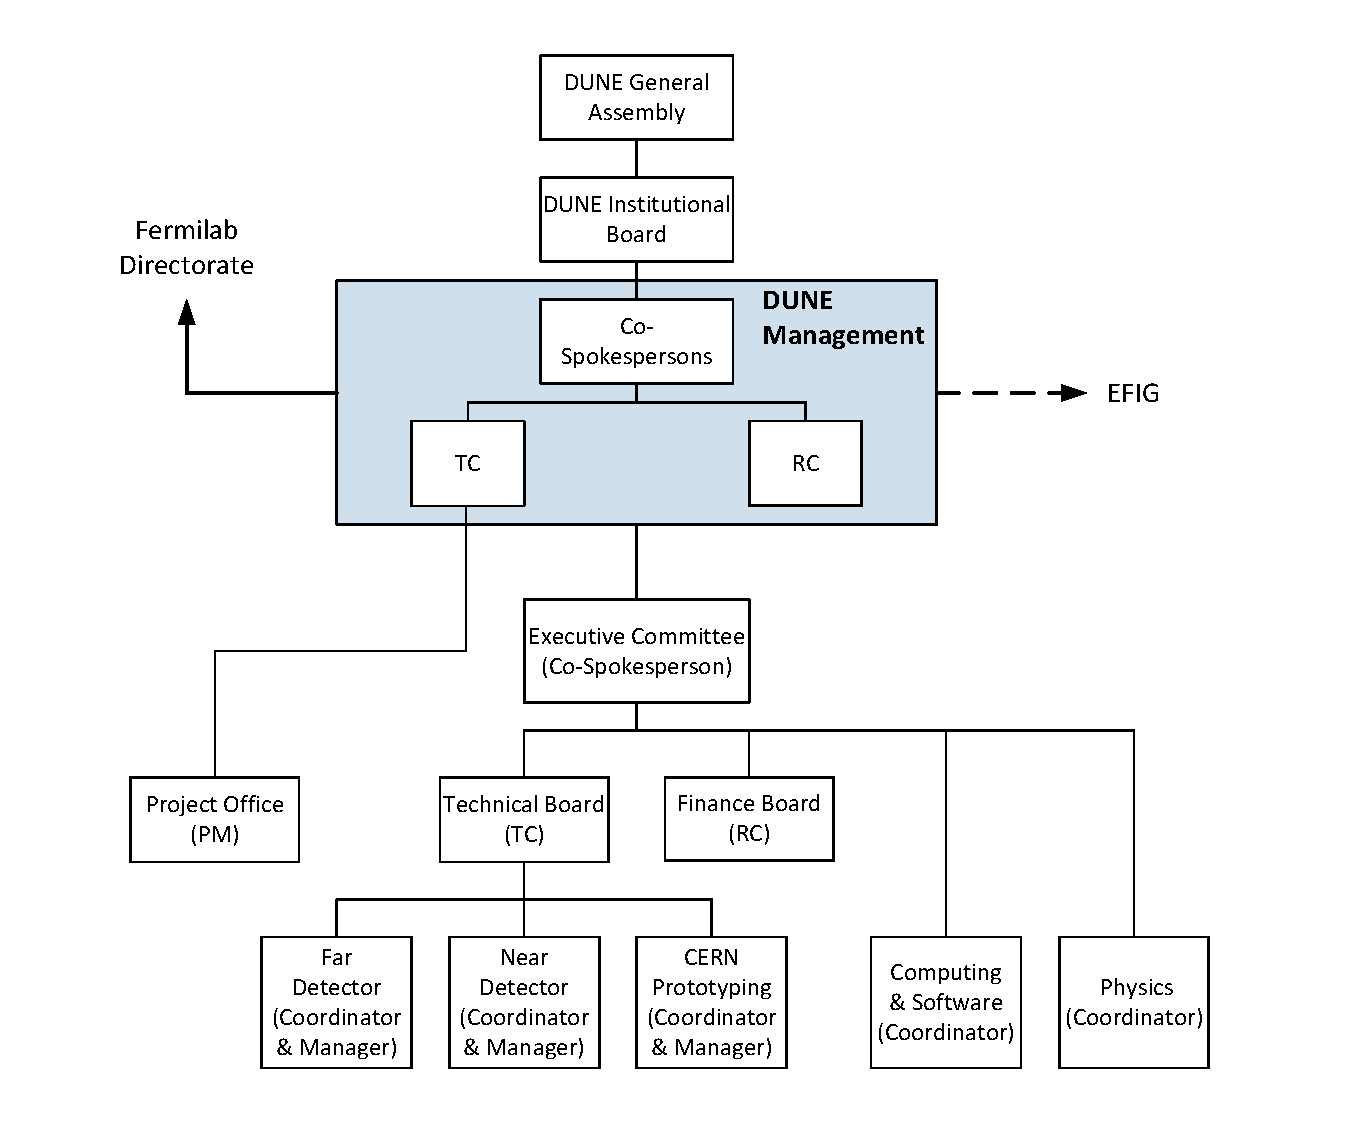
\includegraphics[scale=0.7]{figures/150530_DUNE_Collaboration_20150525.pdf}
  \caption{Organization of the DUNE collaboration.}
  \label{fig:DuneOrg}
\end{figure}
%
The international DUNE Project Office is overseen by the Technical Coordinator and coordinates the work packages assigned to each 
of the different international partners contributing to the effort.  The Project Office maintains a schedule covering the entire 
scope of the project (incorporating all of the individual work packages) and tracks progress through a detailed set of milestones 
embedded within this schedule.  The schedule is based on a Work Breakdown Structure (WBS), which within its cascading levels 
incorporates all required components of the detector construction projects.  The highest-level elements within this WBS structure 
encompass multiple work packages assigned to different international partners.  The deliverables associated with individual work 
packages become separated at lower levels within the WBS structure, where the contributions from specific partners are broken out 
as independent WBS elements.

The DUNE Collaboration structure incorporates detector and prototyping organizations that mimic the WBS structure of the project.  
All matters related to the design, construction, installation, and commissioning of individual detector elements are discussed 
within these organizations.  Because these organizations serve as the required interface between the DUNE Collaboration and the 
international DUNE Project, they incorporate both a coordinator who reports to the DUNE Executive Committee through the Technical
Board of the collaboration and a manager who reports to the Project Office.  The coordinators and managers of the organizations  
are also members of the Technical Board, which coordinates activities across organizations and acts on lower-level project change 
control requests.  Coordination of simulation and data analysis activities are the responsibilities of the Computing \& Software 
and Physics Coordinators, respectively, who report directly to the collaboration Executive Committee and manage collaboration 
working groups covering the full scope of activities within their areas.     

As shown in Fig.~\ref{fig:DuneOrg}, the collaboration structure includes a high-level organization focusing specifically on the 
CERN prototyping effort.  The interim coordinator of this group is Thomas Kutter (Louisiana State University) and the interim 
manager is Greg Pawloski (University of Minnesota).  Coordinator responsibilities include defining operational requirements, 
communicating with the CERN SPSC and leaders of the CERN neutrino platform, as well as coordination of all activities associated 
with the installation, commissioning, and operation of the detector in the CERN test beam area.  The design and construction of 
the DUNE-PT is undertaken by the DUNE Far Detector Organization, whose interim coordinator and manager is Jim Stewart (Brookhaven 
National Laboratory).  The DUNE management team oversees all of the collaboration activities related to the design, construction, 
installation, commissioning, and operation of the DUNE-PT through the collaboration Technical Board.

The DUNE Software \& Computing and Physics Coordinators will form collaboration working groups focusing on simulation and data 
analysis efforts related to the CERN-PT.  The current co-leaders of the DUNE effort to develop a comprehensive and prioritized 
list of measurements required to evaluate the performance of the detector and provide the particle response models necessary for 
DUNE sensitivity studies are Donna Naples (University of Pittsburgh) and Jaroslaw Nowak (University of Lancaster).  Complementary 
efforts to define requirements on the test beam necessary for making these measurements and communicating with the CERN beamline 
coordinator on how to implement these requirements are headed by Cheng-Ju Lin (Lawrence Berkeley National Laboratory).  

%The CERN prototype effort is coordinated by the "CERN Prototype Technical Coordinator (CTC)" \cite{LBNEorg}.
%The charge of the CERN prototype Collaboration Technical Coordinator is defined as follows.
%The CERN prototype CTC is responsible for the following:
%
%	\item Prioritize and maintain a schedule of collaboration activities regarding simulations and physics analysis.
%	\item Prioritize and maintain a schedule of other collaboration service activities on the CERN prototype.  These 
%         activities may include collaboration participation in assembly, commissioning, calibration, debugging, data-taking, shifts, etc.
% 	\item The responsibility of the CERN prototype CTC shall include maintaining a database of contributions from the collaboration to 
%         the CERN detector and beam test prototyping.
%	\item The CERN prototype CTC shall recruit collaboration personnel and resources.
%	\item The CERN prototype CTC shall coordinate with the DUNE far detector L-2 project manager and the DUNE technical coordinator
%\end{enumerate}
%There are currently one CTC,Thomas Kutter (LSU)  and a deputy, Greg Pawloski (Minnesota) sharing the responsibilities.\\
 
%In order to effectively execute the tasks required for the CERN prototype detector and beam test several sub-groups have been created 
%and sub-group leaders have been appointed.

%{\bf Measurement Program + Analysis :}   Their charge is to develop a comprehensive and prioritized list of measurements required to 
%   evaluate detector performance and provide detector charged particle response as input into DUNE physics sensitivity studies (beam 
%physics, nucleon decay, supernovae, atmospheric neutrinos).  And to perform simulation studies to quantitatively compare the relevance 
%of various measurements.  The leaders are Donna Naples (Pittsburgh) and Jaroslaw Nowak (Lancaster).
 
 
%{\bf Beam :} Their charge is to work closely with the measurement group to identify ideal beam requirements, to work closely with the CERN
%beam group to develop realistic beam design to make relevant beam measurements, to evaluate and optimize possible beam injection points and 
%beam orientations, to perform beam simulations and provide simulated beam spectra as input for detector response simulations, to identify 
%required beam instrumentation for beam characterization, and to develop beam run plans.  The  beam subgroup leader is Cheng-Ju Lin (LBNL).


%{\bf Calibration :}  Their charge is to develop tools to calibrate the performance of the detector, to interface with the physics measurement 
%group to prioritize different calibration measurements, and to interface with detector subcomponent working groups to identify all required 
%calibration tools and their integration into the detector /cryostat design.
%The calibration sub-group leaders are Qiuguang Liu (LANL) [interim] and Michele Weber (Bern).\\


%The CERN prototype coordinators work closely with the DUNE technical coordinator and the DUNE far detector manager.
%Direct communication with  DUNE spokespeople is important for any strategic issues.
%The CTC also coordinates closely with the CERN Neutrino Platform leader.
%The leaders of the "measurement program + analysis" subgroup work closely with the DUNE physics and software tools working group leaders. 
%The leader of the "beam" subgroup works closely with the relevant CERN beam-line group leader.

\subsection{Schedule}

The proposed schedule for constructing, installing, and operating the DUNE-PT is driven by the desire of the DUNE collaboration to 
complete these activities on a timescale that will inform construction of the the first 10~kt detector module at SURF, which has 
a scheduled installation beginning in early 2022.  For this reason, the collaboration would ideally like to fully commission the 
detector and collect data for analysis prior to 2019.  However, the primary collaboration goal of validating the design for the 
first 10~kt detector module at SURF can be mostly accomplished through the collection of cosmic ray data.  Therefore, although 
it would be highly preferable to collect beam data prior to 2019, data collected after this date would still be available in time 
to play its essential role in understanding the data to be collected from the first 10~kt detector at SURF.   

A schedule that allows for the collection of test beam data prior to 2019 is shown in Fig.~\ref{fig:schedule}.  Detector construction 
is scheduled to begin in the second quarter of 2016 and the modules would be transported to CERN in two batches so that installation 
at the test beam site could begin as soon as the cryogenic infrastructure including the detector cryostat was available.  Using 
this approach, the detector installation, which is expected to require a little under one year to complete, could be finished by 
the beginning of 2018, allowing for an early-2018 filling of the cryostat and a short data run prior to the shutdown.  Detector 
construction times are informed by recent experience obtained from building prototype detector modules for the 35~t cryostat at 
Fermilab, which will start taking cosmic ray data in the fall of 2015.          

\begin{figure}[htb]
  \centering
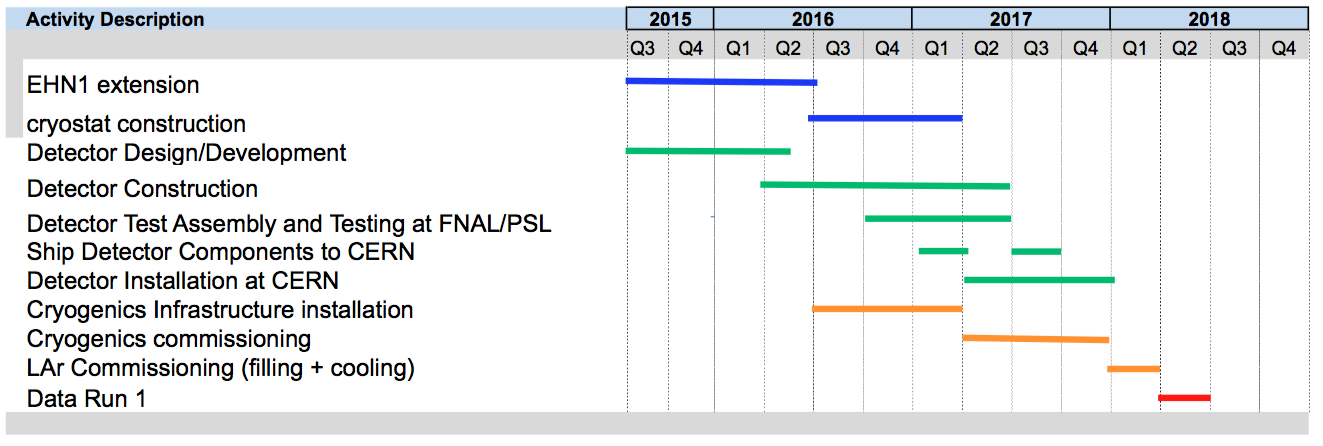
\includegraphics[scale=0.34]{figures/150529_CERNproto_schedule.png}
  \caption{Rolled up version of a draft schedule for DUNE-PT. A 2 - 3 months data taking period is included in the schedule. }
  \label{fig:schedule}
\end{figure}

%The major milestones for the proposed CERN prototype detector construction and beam test is dictated by the DUNE overall schedule which 
%foresees to place the first 10~kton detector module underground as early as calendar year 2021. Additional detector modules, possibly of
%different design, are expected to follow at intervals of 1-2 years in a technically driven schedule.  Information and experience gained 
%from manufacturing, installing and operating the CERN detector test will inform decision regarding future DUNE far detectors.
%The LHC long shutdown, which is presently scheduled for mid-2018 represents a significant constraint on the beam data run schedule.
%Cosmic muon data taking and ideally also beam data taking for the proposed measurement program 
%should be acquired prior to  the long LHC shutdown in mid-2018. While it is desirable to have results from the charged particle beam run 
%available as soon as possible the value of these results is not diminished if they become available only after installation of the DUNE 
%far detector.
%Figure \ref{fig:schedule} shows a technically limited schedule which meets the above requirements.
%is based on experiences from the production and installation schedule for the 35~t detector.
%This schedule is based on experience of designing and manufacturing components for the 35t detector which will be commissioned starting 
%in August 2015 at  Fermilab.
%
%
%Pending an approval of the effort proposed in this document we foresee the following milestones
%\begin{itemize}
%\item early 2017: Cryostat constructed
%\item early 2016: TPC production readiness review
%\item 2016/2017: Engineering Trial Detector Assembly
%\item 2017/2018: Detector Installation
%\item 2018: Detector commissioning 
%\end{itemize}

\subsection{Institutional Responsibilities}

The deliverables required to construct and operate the DUNE-PT are summarized in table~\ref{tab:wbs-detector}.  DUNE is a new collaboration 
recently organized to incorporate former members of the LBNE and LBNO collaborations and other interested members into a unified 
effort to perform the best possible measurements of neutrino oscillations, proton decay, and supernova neutrinos using large-scale, 
deep-undergound liquid argon detectors.  Institutional responsibilities for specific detector construction activities are still 
under development.  In table~\ref{tab:wbs-detector}, DUNE institutions expected to contribute to the production of specific detector elements 
needed for the DUNE-PT are listed. 
%
\begin{table}[h]
\centering
\begin{tabular}{|l l c|}
\hline
\textbf{item no. } & \textbf{Deliverable}  & \textbf{Contributing Institutes}  \\ \hline

1.   & Single-phase LAr detector & \\
1.1  & TPC & BNL, CERN, Lancaster, LBNL, Liverpool \\
  &  & Manchester, Princeton, Sheffield, Wisconsin \\
1.2  & Cold electronics  & BNL, Fermilab, Penn, SMU \\ 
1.3  & Photon detection system  &  ANL, Campinas, CSU, Hawaii, IU, LSU \\
1.4  & DAQ & Cambridge, Duluth,  Fermilab, LANL \\
       &          & Oxford, SLAC \\
1.5  & HV power supplies \& feedthroughs  &  ETHZ, UCLA \\
1.6  & Installation & CERN, Duke, Fermilab, Minnesota \\ 
1.7  & Interfaces  & BNL, LBNL, CERN, Fermilab  \\ \hline

2.   & Operation \& Scientific Effort & \\ 
2.1 & Operation & DUNE-PT collaborators \\
2.2  & Software \& Simulations &  DUNE \\
2.3  & Data analysis &  DUNE \\ \hline

\end{tabular}
\caption{List of work packages and deliverables for detector components and scientific effort.} 
\label{tab:wbs-detector}
\end{table}
%
 It should be noted that the participation of some institutions on this list is dependent on 
the acceptance of recently-submitted or future funding requests from their supporting agencies.  A high priority for the DUNE 
collaboration management moving forward will be to finalize a matrix of responsibilities among the collaborating institutions.  It 
is expected that this process will lead to a significant increase in the level of effort associated with the development of all 
required detector components.  In the meantime, the institutions who have been involved in the proposed design of the DUNE-PT
will be expected to push the effort forward during this transition period to ensure that the collaboration is able to maintain the 
proposed schedule for having detectors installed at CERN in early 2018.

Although the construction, installation, and operation of the DUNE-PT will be the responsibility of the DUNE collaboration, we do 
ask for support from the CERN neutrino platform in the form of detector infrastructure as summarized in table~\ref{tab:wbs-infra}.  
%
\begin{table}[h]
\centering
\begin{tabular}{|l l c|}
\hline
\textbf{item no. } & \textbf{Deliverable}  & \textbf{Contributing Institutes}  \\ \hline

3.   & Detector Infrastructure \& Beam & \\
3.1  & Cryostat &  CERN \\
3.2  & Cryogenics system   &  CERN \\
3.3  & Infrastructure  & CERN \\ 
3.4 & Beam & CERN \\ \hline

\end{tabular}
\caption{List of work packages and deliverables for infrastructure.} 
\label{tab:wbs-infra}
\end{table}
%
In particular, we ask for support for the 
construction and installation of the cryostat and supporting cryogenic systems needed to house and operate the experiment as well 
as access to common infrastructure within the CERN test beam area such as slow controls and data concatenation systems.  We also 
request support from the CERN accelerator departments to provide the required beamline.

Construction, installation, and operation of the DUNE-PT will be conducted following all Fermilab and CERN safety regulations.  
DUNE management has direct line responsibility for safety and is assisted in this effort by the DUNE project ES\&H manager, 
Mike Andrews (Fermilab). 
              
%The deliverables for the CERN single phase prototype detector down to level 3, associated DUNE project 
%work break down structure (WBS)  numbers and contributing institutions are shown in table~\ref{tab:wbs}.





%
%Work on a MOU between the CERN nu-platform and DUNE describing responsibilities, listing institutions 
%involved and defining deliverables has started. 

\subsection{Cost estimate and funding sources}
Cost estimates in {\bf core}  accounting of the various detector components and infrastructure items that 
will be provided for the DUNE-PT by the particpating members of the DUNE collaboartion are shown in 
table~\ref{tab:cost}.  Core M\&S cost estimates do include the cost of the labor hours required to 
assemble and install the various detector components, which are separately provided.  Costing of the 
various detector components is informed by the previously mentioned construction activities associated 
with building prototype detectors for the 35~t cryostat at Fermilab.

Financial support for the construction and installation of the DUNE-PT will be obtained through the 
funding agencies of the various institutions involved in the effort.  Current funding available for 
the effort is via the DUNE US project supported by the United States Department of Energy (DOE).  It 
is expected that additional funding sources associated with non-DOE insitutions will be obtained for 
this effort within the next year.  However, even if this does not occur, the funding profile for the 
DUNE US project over the next three years is by itself sufficient for supporting DUNE responsibilities 
to the DUNE-PT, which the collaboration is supporting as its highest priority activity during this 
time period.      
  
%The total estimated cost of the CERN single phase LAr prototype detector is presented in .
%Cost figures are informed by component production for the 35~t detector.

\begin{table}[h!]
\centering
\begin{tabular}{| l| c| c |}
\hline
\textbf{Detector Element} & \textbf{core M\&S Cost }  & \textbf{core Labor}  \\
 & \textbf{ [US \$]}  & \textbf{ [hours]}  \\ \hline
Time Projection Chamber & 1,210,000 & 6,200 \\
Cold Electronics & 1,260,000 & 4,500 \\
Photon Detection System & 610,000 & 4,200 \\
DAQ & 100,000 & 1,700 \\
HV power supplies & 300,000 & 300 \\
Installation \& Commissioning & 30,000 & 12,400 \\ 
Interfaces & 110,000 & 2,500 \\ \hline 
\textbf{Totals} & 3,620,000 & 31,800 \\ \hline
\end{tabular}
\caption{Estimated core costs and labor hours for the main DUNE-PT detector elements to be provided 
by the DUNE Collaboration}
\label{tab:cost}
\end{table}


%\subsection{Division of Responsibilities}

%\subsubsection{Shared responsibilities}

%The engineering design of the cryostat and the cryogenics system is considered to be a shared responsibility between DUNE/LBNF and CERN.


%\begin{itemize}

%\item plans for data analysis and publications:\\
%include: description of overlap/commonalities with WA105 data analysis and joined efforts
%\end{itemize}




%\subsubsection{CERN responsibilities}

%\paragraph{The beam line:} design, setup of the beam line and beam monitoring instrumentation are expected to be provided by CERN.

%\paragraph{The cryostat and cryogenics system:} are expected to be organized and paid for by the CERN nu-platform.
%The scope of the EHN1 cryostat subsystem includes the design, procurement, fabrication, testing, delivery and oversight of a cryostat to contain the liquid argon and the TPC.\\

%\paragraph{DAQ requests:}  Data links of sufficient bandwidth to transfer the data files from the CENF to the CERN data center, and from there to locations worldwide for analysis. \\

%\paragraph{Computing/Software support:} In order to leverage existing software and expertise, appropriate manpower will need to be allocated in order to create and maintain the computing infrastructure necessary for effective use of the reconstruction and physics analysis tools.\\



